\chapter{\label{ch:2-methods}Methods}

\graphicspath{{figures/ch2/}}

\minitoc 

\section{Molecular biology.}
Human Kir6.2 and SUR1 were subcloned into pcDNA4/TO and pCGFP\_EU vectors for expression of wild-type and GFP-tagged constructs, respectively.
pcDNA4/TO and pANAP were obtained from Addgene.
peRF1-E55D and pCGFP\_EU were kind gifts from the Chin Laboratory (MRC Laboratory of Molecular Biology, Cambridge, UK) and the Gouaux Laboratory (Vollum Institute, Oregon, USA) respectively.
Amber stop codons and point mutations were introduced using the QuikChange XL system (Stratagene; San Diego, CA).
All constructs were confirmed by DNA sequencing (DNA Sequencing and Services, University of Dundee, Scotland).

\section{Cell culture and channel expression}
HEK-293T cells were obtained from and verified/tested for mycoplasma by LGC standards (ATTC CRL-3216, Middlesex, UK).
Our working stock tested negative for mycoplasma contamination using the MycoAlert Mycoplasma Detection Kit (Lonza Bioscience; Burton on Trent, UK).
Cells were plated onto either poly-L-lysine coated borosilicate glass coverslips (VWR International; Radnor, PA) or poly-D-lysine coated glass-bottomed FluoroDishes (FD35-PDL-100, World Precision Instruments).
ANAP-tagged Kir6.2 constructs were labelled using amber stop codon suppression as described in reference \cite{chatterjee_genetically_2013}.
Transfections were carried out 24 hours after plating using TransIT-LT1 (Mirus Bio LLC; Madison, WI) at a ratio of 3 \si{\micro\litre} per \si{\micro\gram} of DNA.
Unless specified otherwise, all transfections included a Kir6.2 construct with an amber stop codon (TAG) at position 311 (Kir6.2-W311\textsuperscript{TAG}), SUR1, pANAP and eRF1-E55D in the ratio 0.5:1.5:1:1.
Transfected cells cultured in Dulbecco’s Modified Eagle Medium (Sigma; St. Louis, MO) + 10\% foetal bovine serum, \SI{100}{\Unit\per\milli\litre} penicillin and \SI{100}{\micro\gram\per\milli\litre} streptomycin (Thermo Fisher Scientific; Waltham, MA) supplemented with \SI{20}{\milli\Molar} ANAP (free acid, AsisChem; Waltham, MA).
Cells were incubated at \SI{33}{\degreeCelsius} and in the presence of \SI{300}{\micro\Molar} tolbutamide to enhance protein expression and channel trafficking to the plasma membrane \cite{yan_sulfonylureas_2004, martin_pharmacological_2013}.
eRF1-E55D was included to increase efficiency of ANAP incorporation.
Experiments were carried out 2-4 days after transfection.
We also expressed constructs labelled with ANAP at positions I182, F183, F198, and I210.
Kir6.2-F183*, Kir6.2-F198*, and Kir6.2-I210* co-expressed with SUR1 did not produce sufficient currents for subsequent experimentation.
Mutations at I182 are known to produce profound effects on nucleotide inhibition of K\textsubscript{ATP}.
Thus, we did not consider this site for further experimentation.

\section{Western blots}
Transfected HEK-293T cells grown in 6-well plates were harvested in cold PBS (Life Technologies Limited; Paisley, UK), pelleted at 0.2 x g for 2.5 minutes and resuspended in lysis buffer containing \SI{0.5}{\percent} Triton X-100, \SI{100}{\milli\Molar} potassium acetate, and a cOmplete protease inhibitor tablet (1 tablet/\SI{50}{\milli\litre}, Roche; Basel, Switzerland), buffered to pH 7.4.
After a 30-minute benzonase (Sigma) treatment at room temperature, samples were mixed with a DTT containing reducing agent and loading buffer (NuPAGE, Invitrogen; Carlsbad, CA) and run on a precast Bis-Tris \SIrange{4}{12}{\percent} poly-acrylamide gel at \SI{200}{\volt} for 40 minutes.
Proteins were wet transferred overnight onto polyvinylidene difluoride (PVDF) membranes (Immobilon P, Merck Millipore; Burlington, VT) in \SI{25}{\milli\Molar} Tris, \SI{192}{\milli\Molar} glycine, \SI{20}{\percent} methanol, and \SI{0.1}{\percent} SDS at \SI{10}{\volt} on ice.
Membranes were blocked with \SI{5}{\percent} milk in TBS-Tw (\SI{150}{\milli\Molar} NaCl, \SI{0.05}{\percent} Tween 20, \SI{25}{\milli\Molar} Tris, pH 7.2) before staining for 30 minutes with a 1:1000 dilution of rat anti-HA monoclonal antibody in TBS-Tw (clone 3F10, Roche).
After washing with TBS-Tw, membranes were incubated for 30 minutes with a 1:20,000 dilution of HRP-conjugated goat anti-rat polyclonal antibodies in TBS-Tw (Jackson ImmunoResearch; Ely, UK).
Detection was performed using the SuperSignal West Pico Chemiluminescent Substrate (Thermo Fisher) and a C-DiGit Blot Scanner (Licor Biosciences; Lincoln, NE).
Analysis was performed using custom code written in Python.

To confirm our ability to express full-length W311*-GFP, we performed western blots for HA-tagged Kir6.2 constructs in detergent-solubilized HEK-293T cells (Figure \ref{ch3fig:western_1}).
The HA tag plus a short linker (YAYMEKGITDLAYPYDVPDY) was inserted in the extracellular region following helix M1 of Kir6.2 between L100 and A101.
Transfection of wild-type Kir6.2-HA or Kir6.2-HA-GFP resulted in two bands on the western blots.
The upper bands were close to the expected sizes for full-length Kir6.2-HA and Kir6.2-HA-GFP (\SI{46}{\kilo\dalton} and \SI{77}{\kilo\dalton}, respectively).

We consistently observed a lower molecular weight band as well.
This band must correspond to an N-terminally truncated Kir6.2 product, as the apparent molecular weight shifted with addition of the C-terminal GFP tag.
Based on the molecular weight, we predict that the truncated protein product initiated from a start codon in the first transmembrane domain.
Therefore, we believe it is unlikely that this protein would form functional channels or traffic to the plasma membrane.
When Kir6.2-W311\textsuperscript{TAG}-HA or Kir6.2-W311\textsuperscript{TAG}-HA-GFP were co-transfected with SUR1, pANAP, and eRF1-E55D, and cells were cultured in the presence of ANAP, the western blots were similar to wild-type Kir6.2-HA or Kir6.2-HA-GFP.
Over \SI{90}{\percent} full-length W311*-HA-GFP was produced under these conditions.
We were unable to quantify the percentage of full-length W311*-HA produced as the C-terminally truncated band resulting from termination at the TAG codon was very similar in size to the N-terminally truncated band.
Co-expression with SUR1 increased the percentage of full-length W311*-HA-GFP produced.
In the absence of ANAP, we did not observe any full-length Kir6.2, indicating that there was no read-through of the amber (TAG) stop codon.

\section{Confocal microscopy}
Confocal imaging was performed using a spinning-disk system (Ultra-VIEW VoX, PerkinElmer; Waltham, MA) mounted on an IX81 microscope (Olympus; Southend-on-Sea, UK) with a Plan Apo 60x oil immersion objective (NA = 1.4), provided by the Micron Advanced Bioimaging Unit, Oxford.
Transfected HEK-293T cells were incubated for 15 minutes with \SI{1}{\nano\Molar} CellMask Deep Red (Thermo Fisher) to stain plasma membranes before washing with PBS and imaging.
ANAP was excited with a solid-state laser at \SI{405}{\nano\Molar}.
GFP and CellMask were excited with an argon laser at \SI{488}{\nano\Molar} and \SI{633}{\nano\Molar} respectively.
Images were captured on an EMCCD camera (ImagEM; Hamamatsu Photonics; Welwyn Garden City, UK) binned at 2 x 2 pixels and analysed using Python.
A median filter with a box size of 32 x 32 pixels was applied to improve the signal-to-noise ratio by reducing background fluorescence.

We examined the surface expression of our ANAP-labelled constructs using confocal microscopy.
When Kir6.2-W311\textsuperscript{TAG}-GFP was co-transfected with SUR1 along with pANAP and eRF1-E55D in the presence of ANAP, the ANAP and GFP fluorescence were co-localized at the plasma membrane.
When wild-type Kir6.2-GFP was transfected under the same conditions, only GFP fluorescence was observed at the plasma membrane.
ANAP fluorescence was diffuse and confined to the cytoplasm or intracellular structures.
Thus, the plasma-membrane ANAP signal was specific for W311*-GFP.

\section{Surface expression assays}
We measured surface expression of HA-tagged Kir6.2 subunits using an approach outlined by Zerangue et al.
Cells were plated on \SI{19}{\milli\metre} coverslips coated with poly-L-lysine and transfected as described above.
Following incubation, cells were rinsed with PBS before fixation with \SI{10}{\percent} formalin for 30 minutes at room temperature.
After washing again, cells were blocked with \SI{1}{\percent} BSA in PBS for 30 minutes at \SI{4}{\degreeCelsius} before a 1-hour incubation at \SI{4}{\degreeCelsius} with a 1:1000 dilution (in PBS) of rat anti-HA monoclonal antibodies.
Cells were then washed 5 times on ice with \SI{1}{\percent} BSA in PBS followed by a 30-minute incubation at \SI{4}{\degreeCelsius} with a 1:2000 dilution of HRP-conjugated goat anti-rat polyclonal antibodies.
Cells were washed 5 times in PBS + \SI{1}{\percent} BSA and 4 times in PBS.
Coverslips were removed from the culture dishes and placed in clean, untreated dishes for measurement.
\SI{300}{\micro\litre} of SuperSignal ELISA Femto Maximum Sensitivity Substrate (Thermo Fisher) was added to each sample and the luminescence was measured using a Glomax 20/20 Luminometer (Promega; Madison, WI) after a 10 second incubation.

HEK-293T cells were transfected with Kir6.2 constructs with or without a TAG stop codon corresponding to position 311.
Cells were co-transfected with pANAP and eRF1-E55D in the presence or absence of SUR1 and cultured with or without ANAP.
Wild-type Kir6.2-HA and Kir6.2-HA-GFP in the presence of SUR1 were included as positive controls.
Kir6.2 constructs with no HA tag served as negative controls.
In the presence of ANAP, we observed strong trafficking of W311*-HA-GFP to the plasma membrane, but much less trafficking of W311*-HA (Figure 1—Figure supplement 1E).
When cells were cultured in the absence of ANAP, we observed little to no Kir6.2 surface expression from cells that were transfected with Kir6.2-W311\textsuperscript{TAG}-HA or Kir6.2-W311\textsuperscript{TAG}-HA-GFP, suggesting that prematurely truncated constructs did not traffic to the plasma membrane.
In the absence of SUR1, surface expression was weak for both wild-type and tagged constructs, despite the reported ability of Kir6.2-GFP to traffic to the plasma membrane in the absence of SUR1.

\section{Epifluorescence imaging and spectroscopy}
Epifluorescence imaging and spectroscopy were performed using a Nikon Eclipse TE2000-U microscope with a 60x water immersion objective (Plan Apo VC, NA = 1.2, Nikon; Kingston upon Thames, UK) or a 100x oil immersion objective (Nikon, Apo TIRF, NA = 1.49).
Imaging of ANAP was performed using a \SI{385}{\nano\metre} LED source (ThorLabs; Newton, NJ) with a \SI{390/18}{\nano\metre} band-pass excitation filter, an MD416 dichroic and a \SI{479/40}{\nano\metre} band-pass emission filter (all from ThorLabs).
GFP was imaged using a \SI{490}{\nano\metre} LED source (ThorLabs) with a \SI{480/40}{\nano\metre} band-pass excitation filter, a DM505 dichroic, and a \SI{510}{\nano\metre} long-pass emission filter (all from Chroma; Bellows Falls, VT).
Fluorescence spectra were collected by exciting ANAP as above but using a \SI{400}{\nano\metre} long-pass emission filter (ThorLabs), then passing emitted light through an IsoPlane 160 Spectrometer (Princeton Instruments; Trenton, NJ) with a \SI{300}{\gram\per\milli\metre} grating.
Images were collected with \SI{1}{\second} exposures on a Pixis 400BR\_eXcelon CCD (Princeton Instruments).

\section{Electrophysiology.}
Patch pipettes were pulled from thick-walled borosilicate glass capillaries (GC150F-15, Harvard Apparatus; Holliston, MA) to a resistance of \SIrange{1.5}{2.5}{\mega\ohm} when filled with pipette solution.
Currents were recorded at \SI{-60}{\milli\volt} from excised inside-out patches using an Axopatch 200B amplifier equipped with a Digidata 1322A digitizer and using pClamp 10 software (Molecular Devices; San Jose, CA).
Currents were low-pass filtered at \SI{5}{\kilo\hertz} and digitized at \SI{20}{\kilo\hertz}.
The bath solution (intracellular) contained \SI{140}{\milli\Molar} KCl, \SI{10}{\milli\Molar} HEPES, \SI{1}{\milli\Molar} EDTA and \SI{1}{\milli\Molar} EGTA (pH 7.3 with KOH).
The pipette solution (extracellular) contained \SI{140}{\milli\Molar} KCl, \SI{10}{\milli\Molar} HEPES and \SI{1}{\milli\Molar} EDTA (pH 7.4 with KOH).
All experiments were carried out in Mg\textsuperscript{2+}-free conditions.
Currents were leak corrected using the current remaining in bath solution containing \SI{5}{\milli\Molar} barium chloride at \SI{+60}{\milli\volt}, assuming a linear leak with a reversal potential of \SI{0}{\milli\volt}.
Inhibition was calculated and corrected for rundown by alternating test concentrations of nucleotide solution with nucleotide-free solution, then expressing the test currents as a fraction of the average of the control currents before and after the test solution.

\section{FRET calculations}
We calculated the expected FRET efficiency between ANAP incorporated at amino acid position 311 and a docked TNP-ATP molecule.
The efficiency of energy transfer is exquisitely distance-dependent, and can be calculated with the following formula:
\begin{equation} \label{eq:forster_fret}
E = \frac{1}{1 + \frac{R^6}{R_0^6}}
\end{equation}
where $R$ is the distance between donor and acceptor fluorophores and $R_O$ is a characteristic distance at which \SI{50}{\percent} of the energy is transferred.
We calculated the R0 of the ANAP:TNP-ATP FRET pair using the following equations from \citeauthor{selvin_13_1995}:
\begin{equation} \label{eq:selvin_fret}
\begin{split}
R_0 &= (8.79 \times 10^{-5} J q_D n^{-4} \kappa^2)^{1/6}\\
J &= \frac{\int \epsilon_A (\lambda) f_D (\lambda) \lambda^4 d \lambda}{\int f_D (\lambda) d \lambda}
\end{split}
\end{equation}
where $J$ (in \si{\per\Molar\per\centi\metre\nano\metre}\textsuperscript{4}) is the normalised spectral overlap of the donor emission ($f_D$) and acceptor extinction ($\epsilon_A$), $q_D$ is the quantum efficiency of the donor measured in the absence of the acceptor, $n$ is the refractive index for the medium the experiment is performed in, and $\kappa^2$ is a geometric factor related to the relative orientation of the two transition dipoles of donor and acceptor that can take values between 0 and 4.

For our purposes, we measured the overlap between donor emission measured from the averaged spectra from multiple unroofed membranes containing W311* without the C-terminal GFP tag, and acceptor extinction spectra measured from TNP-ATP in solution using a Beckman Coulter DU800 spectrophotometer (Pasadena, CA).
We did not measure the $q_D$ of ANAP ourselves, instead using the quantum yield of 0.22 measured by \citeauthor{zagotta_measuring_2016}.
As our experiments were performed in a water-based medium, we used the refractive index of water ($n = 1.33$).
We used a $\kappa^2$ value of $\frac{2}{3}$, which is the case when the orientation of dipoles of donor and acceptor are able to rotate freely within the excited state donor lifetime.

The equivalency between FRET efficiency (measured as ANAP quenching) and nucleotide binding is based on two main assumptions.
Firstly, we assume that the observed quenching from a bound nucleotide does not differ dramatically between open and closed states of the channel.
As there is no open-state structure of K\textsubscript{ATP}, we do not know exactly how much relative movement would occur between a bound TNP-ATP and Kir6.2-W311.
However, based on cryo-EM structures of apo and nucleotide-bound Kir6.2 we do not expect to see a change in the distance between these two positions.
Secondly, we assume that the orientation of the ANAP and TNP-ATP dipoles can be well described by a $\kappa^2$ value of $\frac{2}{3}$.
This assumption is commonly made in FRET assays, and reference \cite{stryer_fluorescence_1978} shows that uncertainty introduced by this assumption is relatively small (typically less than \SI{20}{\percent}). Empirically, our results showing FRET occurs to a similar extent as predicted by formula \ref{eq:forster_fret} supports this assumption as reasonable.

\section{Unroofed binding measurements.}
Unroofed membranes were prepared as follows.
A coverslip plated with transfected HEK-293T cells was removed from the culture media and rinsed with PBS.
The coverslip was then briefly sonicated using a probe sonicator (Vibra-cell; Newtown, CT) leaving behind adherent plasma membrane fragments.
Cells cultured on FluoroDishes were rinsed and sonicated directly in the dish.
Unroofed membrane fragments were nearly invisible in bright-field images and identified by the presence of GFP and ANAP fluorescence.
Fluorescent TNP-nucleotides (Jena Bioscience; Jena, Germany) were diluted in bath solution and perfused onto unroofed membranes using a valve controlled microvolume superfusion system (\si{\micro}Flow, ALA Scientific Instruments; Farmingdale, NY).

Fluorescence spectra were collected as described above.
A region of interest corresponding to the membrane fragment was manually selected and line-averaged for each wavelength.
A similarly sized region of background was selected and averaged, then subtracted from the spectrum of interest.
After subtraction, ANAP intensity was calculated by averaging the fluorescence intensity measured between \SI{469.5}{\nano\metre} and \SI{474.5}{\nano\metre}.
Bleaching was corrected by fitting the normalised ANAP intensity of exposures taken during perfusion with nucleotide-free solution to a single exponential decay of the form
\begin{equation} \label{eq:bleaching}
    \frac{F}{F_{max}} = ae^{kt} + (1 - a)
\end{equation}
then using the fit to correct the intensity of exposures taken during perfusion with test nucleotide solutions.

Some experiments were excluded from further analysis due to obvious cross-contamination between different solutions within the \si{\micro}Flow superfusion system.
These were identified by noticeable colour changes in the solution in the delivery tubes.

\section{Patch-clamp fluorometry.}
The tip of the patch pipette was centred on the slit of the spectrometer immediately after patch excision.
Currents were measured as described above.
Fluorescence emission spectra from the excised patch were acquired concurrently with current measurements, both during test solution application as well as nucleotide-free solution.
Background subtraction was slightly imperfect due to the exclusion of TNP-ATP from volume of the glass of the pipette, resulting in spectra that have negative intensities at the TNP-ATP peak at high nucleotide concentrations.
However, this over-subtraction does not affect the size of the ANAP peak, which we used to quantify nucleotide binding.

Some experiments were excluded from further analysis due to low fluorescence intensity, as we were concerned about a low signal to noise ratio influencing our results.

\section{Data processing and presentation.}
Raw spectrographic images and current traces were pre-processed in Python and Clampfit (Axon) before analysis with R.
Where applicable, all experimental data points are displayed in each figure.
To help visualise uncertainty and prevent some data points being hidden, they are arranged with a small amount of horizontal jitter; vertical position remains unaffected.

We fit our fluorescence quenching data with the following equation:
\begin{equation} \label{eq:hill}
    \frac{y}{y_{max}} = 1 - E_{max} + \frac{E_{max}}{1 + 10^{(EC_{50} - [TNPATP]) \cdot h}} + \sigma
\end{equation}
where $y$ represents corrected fluorescence intensity, $EC_{50}$ and $[TNPATP]$ are $\log_{10}$ values, and $\sigma$ is the remaining variance.
For the fluorescence quenching data, $E_{max}$ was fixed to the value obtained from W311*-GFP+SUR1 unroofed experiments (0.1) as explained in more detail in chapter \ref{ch4}.
Current inhibition data were fit to the same equation but with $y$ representing normalised current magnitude, $IC_{50}$ instead of $EC_{50}$, and $I_{max}$ instead of $E_{max}$.

We used the brms package in R to perform a non-linear fit to equation \ref{eq:hill} reformulated as a multilevel (or hierarchical) model.
The parameters in the equation were supplied as:

\begin{minipage}{.5\textwidth}
\centering
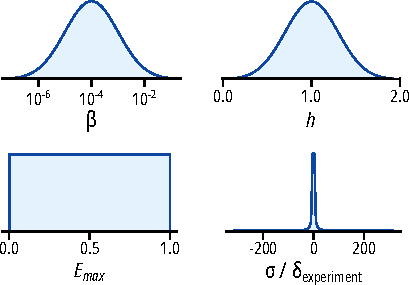
\includegraphics[width=\textwidth]{drc_priors.pdf}
\end{minipage}
\begin{minipage}{.5\textwidth}
\centering
\begin{equation} \label{eq:drc_priors}
\begin{split}
E_{max} &\sim Uniform(0, 1) \\
h &\sim Normal(1, 0.3) \\
EC_{50} &= \beta + \delta_{experiment} \\
\beta &\sim Normal(-4, 1) \\
\delta_{experiment} &\sim Cauchy(0, 1) \\
\sigma &\sim Cauchy(0, 1)
\end{split}
\end{equation}
\end{minipage}

Essentially, the $EC_{50}$ (or $IC_{50}$) parameter for each concentration-response experiment can be described as the combination of a population parameter that is an estimate of the construct-specific value (\textgreek{b}), and an additional 'random' component that varies between experiments on the same construct (\textgreek{d}\textsubscript{experiment}).

Multilevel models seek to describe datasets which consist of clusters or groups of measurements that may differ from one another \cite{andrew_gelman_bayesian_2014, mcelreath_statistical_2020}.
In this case, each cluster of measurements is the set of current inhibition or fluorescence quenching values obtained from a single excised patch or unroofed membrane.
As opposed to fitting each cluster individually, the multilevel model laid out in equation \ref{eq:drc_priors} allows for 'pooling' of information between clusters, so that the parameters for each experiment are influenced by all other experiments on the same construct.
This pooling tends to improve estimates about each cluster.

\section{Model equations and fitting}

The concerted MWC-type model fitted to the patch-clamp fluorometry data was formulated as follows:
\begin{equation} \label{eq:mwc_binding}
\frac{F}{F_{max}} = \frac
    {K_A[TNPATP](1+K_A[TNPATP])^3+LD_AK_A[TNPATP](1+D_AK_A[TNPATP])^3}
    {(1+K_A[TNPATP])^4+L(1+D_AK_A[TNPATP])^4} + \sigma
\end{equation}

\begin{equation} \label{eq:mwc_gating}
\frac{\text{open channels}}{\text{total channels}} = \frac
    {L(1+D_AK_A[TNPATP])^4}
    {(1+K_A[TNPATP])^4+L(1+D_AK_A[TNPATP])^4} + \sigma
\end{equation}

When no ligand is present (i.e. when $[TNPATP] = 0$), equation \ref{eq:mwc_gating} becomes:
\begin{equation} \label{eq:intrinsic_po}
\frac{\text{open channels}}{\text{total channels}} = \frac
    {L}
    {1+L} + \sigma
\end{equation}

We can use this to normalise the predicted changes in the open fraction to an observed change in current:
\begin{equation} \label{eq:normalised_po}
\frac{I}{I_{max}} = \frac
    {L(1+D_AK_A[TNPATP])^4}
    {(1+K_A[TNPATP])^4+L(1+D_AK_A[TNPATP])^4}\cdot
   \frac
    {1+L}
    {L} + \sigma
\end{equation}

We used the brms package in R to fit a multilevel model to equations \ref{eq:mwc_binding} and \ref{eq:normalised_po}.
First, we normalised the fluorescence quenching data by the $E_{max}$ determined from W311*-GFP+SUR1 unroofed experiments (0.1).
We then corrected it by transforming each data point as $log_2(\frac{F}{F_{max} + 1})$ as described in more detail in Chapter \ref{ch3}.

The parameters in the equation were supplied as:

\begin{minipage}{.5\textwidth}
\centering
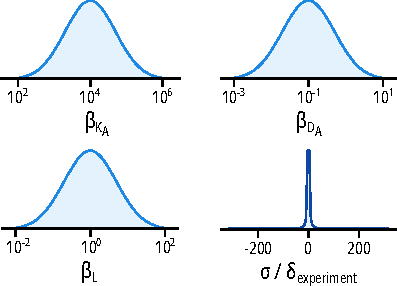
\includegraphics[width=\textwidth]{mwc_priors.pdf}
\end{minipage}
\begin{minipage}{.5\textwidth}
\centering
\begin{equation} \label{eq:mwc_priors}
\begin{split}
log(K_A) &\sim \beta_{K_A} + \delta_{experiment} \\
log(D_A) &\sim \beta_{D_A} + \delta_{experiment} \\
log(L) &\sim \beta_{L} + \delta_{experiment} \\
\beta_{K_A} &\sim Normal(log(10^4), log(5)) \\
\beta_{D_A} &\sim Normal(log(0.1), log(5)) \\
\beta_{L} &\sim Normal(log(1), log(5)) \\
\delta_{experiment} &\sim Cauchy(0, 1) \\
\sigma &\sim Cauchy(0, 1)
\end{split}
\end{equation}
\end{minipage}

Each of the three parameters was modelled as a combination of a population parameter $\beta_x$ and an additional random component $\delta_{experiment}$.
Each combined set of current inhibition and nucleotide binding measurements from one excised patch was grouped as one experiment.
The remaining variance $\sigma$ was allowed to vary between fluorescence and current data.

The alternate single-binding model was formulated as follows:

{\tiny
\begin{equation} \label{eq:single_binding}
\frac{F}{F_{max}} = \frac
{LD_AK_A[TNPATP](1+3K_A[TNPATP]+3K_A^2[TNPATP]^2+K_A^3[TNPATP]^3)+K_A[TNPATP](1+K_A[TNPATP])^3}
{L(1+4D_AK_A[TNPATP]+6D_AK_A^2[TNPATP]^2+4D_AK_A^3[TNPATP]^3+D_AK_A^4[TNPATP]^4)+(1+K_A[TNPATP])^4}
\end{equation}

\begin{equation} \label{eq:single_gating}
\frac{I}{I_{max}} = \frac
{L(1+4D_AK_A[TNPATP]+6D_AK_A^2[TNPATP]^2+4D_AK_A^3[TNPATP]^3+D_AK_A^4[TNPATP]^4}
{L(1+4D_AK_A[TNPATP]+6D_AK_A^2[TNPATP]^2+4D_AK_A^3[TNPATP]^3+D_AK_A^4[TNPATP]^4)+(1+K_A[TNPATP])^4}\cdot\frac
{1+L}
{L}
\end{equation}
}

The extra length of these formulas when compared to equations \ref{eq:mwc_binding} and \ref{eq:normalised_po} do not represent any additional complexity; just an unfortunate consequence of the lack of exponents of $D_A$ which make it impossible to simplify further.
Parameters were supplied and fitted as in equation \ref{eq:mwc_priors}.



\section{Computational docking.}
Computational docking of TNP-ATP into the nucleotide binding site of Kir6.2 was performed using AutoDock-Vina and Pymol (Schrödinger, LLC; New York, NY).
11 TNP-ATP structures from the Protein Data Bank (PDB accession \#s 1I5D, 3AR7, 5NCQ, 5SVQ, 5XW6, 2GVD, 5A3S, 2PMK, and 3B5J) were used as starting poses and a 15x11.25x15 \si{\angstrom} box was centred on the ATP bound to Kir6.2 in PDB accession \#6BAA.
Protonation states for each residue were assigned using PDB2PQR and PROPKA 3.0.
The modal highest-scoring pose from the docking run was selected (PDB accession \#5XW6) and distances were measured from a pseudo atom at the centre of the fluorescent moiety.
TNP-ATP (PDB \#3AR7) was positioned into the first nucleotide binding site of SUR1 (PDB \#6PZI) using the alignment tool in Pymol.

\section{Chemicals and stock solutions.}
Unless otherwise noted, all chemicals were obtained from Sigma.
TNP-ATP was obtained as a \SI{10}{\milli\Molar} aqueous stock from Jena Bioscience and stored at \SI{-20}{\degreeCelsius}. \SI{1}{\milli\Molar} aqueous stocks of ANAP-TFA were prepared by dissolving the free acid in \SI{30}{\milli\Molar} NaOH, and were stored at \SI{-20}{\degreeCelsius}. Tolbutamide stocks (\SI{50}{\milli\Molar}) were prepared in \SI{100}{\milli\Molar} KOH and stored at \SI{-20}{\degreeCelsius}.
